\documentclass[a4paper,oneside,12pt]{article}
\usepackage{graphics,multicol}
\usepackage[latin1]{inputenc}
\usepackage[a4paper,margin=2cm,lmargin=2cm,headheight=1pt]{geometry}
\usepackage{fancyhdr}
\usepackage{amsmath,amssymb,amsfonts,amsthm, mathrsfs}
\usepackage{mathtools,bbm}
\usepackage{IEEEtrantools}
\usepackage[]{algorithm2e}
\usepackage{tikz,pgfplots,tkz-graph}
\usepackage{ifthen,calc}
\usepackage{listings,hyperref,float}
\usepackage{epsfig,epstopdf,graphicx}
\usepackage{enumerate}

\pgfplotsset{compat=newest}
\usetikzlibrary{positioning,matrix}
\interdisplaylinepenalty=2500

% Page settings
% \setlength{\oddsidemargin}{0 in}
% \setlength{\evensidemargin}{0 in}
% \setlength{\topmargin}{-0.6 in}
% \setlength{\textwidth}{6.5 in}
% \setlength{\textheight}{8.5 in}
% \setlength{\headsep}{0.75 in}
% \setlength{\parindent}{0 in}
% \setlength{\parskip}{0.1 in}

% Markov symbol X -o- Y
\newcommand{\markov}{\mathrel{\multimap}\joinrel\mathrel{-}\joinrel\mathrel{\mkern-6mu}\joinrel\mathrel{-}}
% Independent & not independent symbol X _||_ Y
\newcommand{\indep}{\mathrel{\bot}\joinrel\mathrel{\mkern-5mu}\joinrel\mathrel{\bot}}
\newcommand{\dep}{\centernot\indep}
% i.i.d.
\newcommand{\iid}{\stackrel{\mathrm{i.i.d.}}{\sim}}
% Integration d
\newcommand{\dd}{\mathop{}\!\mathrm{d}}

% Single braces
\newcommand{\agbrs}[1]{\left\langle #1 \right\rangle}	% angle braces,  	< x >
\newcommand{\rdbrs}[1]{\left( #1 \right)}				% round braces,  	( x )
\newcommand{\sqbrs}[1]{\left\lbrack #1 \right\rbrack}	% square braces, 	[ x ]
\newcommand{\clbrs}[1]{\left\lbrace #1 \right\rbrace}	% curly braces, 	{ x }

% Delimited braces
\newcommand{\agbrsv}[2]{\left\lange #1 \,\middle|\, #2 \right\rangle}	% angle braces with delimiter |,  	< x | y >, inner product
\newcommand{\rdbrsv}[2]{\left( #1 \,\middle|\, #2 \right)}				% round braces with delimiter |,  	( x | y ), conditional probability
\newcommand{\sqbrsv}[2]{\left\lbrack #1 \,\middle|\, #2 \right\rbrack}	% square braces with delimiter |,  	[ x | y ], conditional expectation
\newcommand{\clbrsv}[2]{\left\lbrace #1 \,\middle|\, #2 \right\rbrace}	% curly braces with delimiter |,  	{ x | y }, set

% Short for underline and overline
\newcommand{\udl}[1]{\underline{#1}}
\newcommand{\ovl}[1]{\overline{#1}}

% Derivative and partial derivation
\newcommand{\fracd}[2]{ \frac{\mathrm{d} #1}{\mathrm{d} #2} }
\newcommand{\fracp}[2]{ \frac{\partial #1}{\partial #2} }

% Absolute value, norm, ceil, floor, and evaluation
\newcommand{\abs}[1]{\left| #1 \right|}		% Absolute value, 	| x |
\newcommand{\norm}[1]{\left\| #1 \right\|}	% Norm, 			|| x ||
\DeclarePairedDelimiter\ceil{\lceil}{\rceil}
\DeclarePairedDelimiter\floor{\lfloor}{\rfloor}
\newcommand{\eval}[1]{\left. #1 \right|}	% Evaluation, 		f(x) |_{x=x0}

% Definition equal sign
\newcommand{\defeq}{\vcentcolon=}   % :=
\newcommand{\eqdef}{=\vcentcolon}   % =:
\newcommand{\texteq}[1]{\stackrel{#1}{=\joinrel=\joinrel=}}   % use for change of variable

% Inverse hyperbolic functions
\DeclareMathOperator\arcsinh{arcsinh}
\DeclareMathOperator\arccosh{arccosh}
\DeclareMathOperator\arctanh{arctanh}
\DeclareMathOperator\atanh{atanh}
\DeclareMathOperator\sech{sech}

% argmax and argmin
\newcommand\limit[1]{\underset{#1}{\lim}\,}
\newcommand\argmax[1]{\mathrm{arg}\,\underset{#1}{\max}\,}
\newcommand\argmin[1]{\mathrm{arg}\,\underset{#1}{\min}\,}

% Matrices
\newcommand*\pmtx[1]{\begin{pmatrix}#1\end{pmatrix}}			% Matrix with round braces
\newcommand*\bmtx[1]{\begin{bmatrix}#1\end{bmatrix}}			% Matrix with square braces
\newcommand*\vmtx[1]{\begin{vmatrix}#1\end{vmatrix}}			% Determinant of matrix
\newcommand*\spmtx[1]{\rdbrs{\begin{smallmatrix}#1\end{smallmatrix}}}	% Small matrix with round braces
\newcommand*\sbmtx[1]{\sqbrs{\begin{smallmatrix}#1\end{smallmatrix}}}	% Small matrix with square braces
\newcommand*\svmtx[1]{\abs{\begin{smallmatrix}#1\end{smallmatrix}}}		% Determinant of small matrix
\newcommand{\sizecorr}[1]{\makebox[0cm]{\phantom{$\displaystyle #1$}}}	% Get size of an expression

% Theorem environments
\newtheorem{theorem}{Theorem}
\newtheorem{corollary}[theorem]{Corollary}
\newtheorem{lemma}[theorem]{Lemma}
\newtheorem{observation}[theorem]{Observation}
\newtheorem{proposition}[theorem]{Proposition}
\newtheorem{definition}[theorem]{Definition}
\newtheorem{claim}[theorem]{Claim}
\newtheorem{fact}[theorem]{Fact}
\newtheorem{assumption}[theorem]{Assumption}

\newtheorem*{theorem*}{Theorem}
\newtheorem*{corollary*}{Corollary}
\newtheorem*{lemma*}{Lemma}
\newtheorem*{proposition*}{Proposition}
\newtheorem*{definition*}{Definition}
\newtheorem*{example*}{Example}
\newtheorem*{remark*}{Remark}
\newtheorem*{problem*}{Problem}

% Solution environment
\newenvironment{solution}{\begin{proof}[Solution]}{\end{proof}}

% Short for boldsymbol
\newcommand{\bs}[1]{\boldsymbol{#1}}

% Other frequent used operators
\def\Var{\mathsf{Var}}
\def\Cov{\mathsf{Cov}}
\def\coeff{\mathsf{coeff}}
\def\Tr{\mathsf{Tr}}
\def\rank{\mathsf{rank}}
\def\diag{\mathsf{diag}}
\def\mse{\mathsf{mse}}
\def\mmse{\mathsf{mmse}}

\def\ee{\mathbbm{e}}
\def\ii{\mathbbm{i}}
\def\EE{\mathsf{E}}
\def\FF{\mathsf{F}}
\def\SS{\mathsf{S}}
\def\UU{\mathsf{U}}
\def\xx{\mathsf{x}}
\def\pprime{{\prime\prime}}

\newcommand{\KL}[2]{D\left( #1 \,\middle|\middle|\, #2 \right)}%                   ( | )

\makeatletter
\newcommand\ztag[1]{%
\def\@currentlabel{#1}%
\gdef\tmp{%
\addtocounter{equation}{-1}%
\def\theequation{#1}}%
\aftergroup\aftergroup\aftergroup\aftergroup\aftergroup\aftergroup
\aftergroup\aftergroup\aftergroup\aftergroup\aftergroup\aftergroup
\aftergroup\aftergroup\aftergroup\aftergroup\aftergroup\aftergroup
\aftergroup\aftergroup\aftergroup\aftergroup\aftergroup\aftergroup
\aftergroup\aftergroup\aftergroup\aftergroup\aftergroup\aftergroup
\aftergroup
\tmp\IEEEyesnumber}


\pagestyle{empty}
\begin{document}

\noindent

\begin{tabular}{lcr}
  Duke University & & Math 690-40 \\  
  Homework one & \hspace{6.3cm} & F. Krzakala and L. Zdeborova\\ \hline
\end{tabular}

\begin{center}
  {\Large {\bf Graphical models and the Ising model}}
\end{center}

\section*{More on matchings:  imposing constraints}

Let's get back to one of our previous homework the matching problem. 
We remind: Given a  (unweighted, undirected) graph $ G(V,E) $ a matching $ \mathsf{M} \in E $ is defined as a subset of edges such that if $ (ij) \in \mathsf{M} $ then no other edge that contains node $ i $ or $ j $ can be in $ \mathsf{M} $. 
In other words a matching is a subset of edges such that no two edges of the set share a node. 
The size of a matching is simply $ \abs{\mathsf{M}} $. 
\begin{enumerate}[(a)]
\item 
        Last time you represented this problem via a graphical model. 
        It is crucial to realize that usually there are several possible ways to do it. 

        This time the task is to write a graphical model for matchings such that if the original graph is a tree (i.e. has no loops) then also the graphical model is a tree (i.e. has no cycles when seen as a simple bipartite graph). 

        Hint: Factor nodes can have more than two neighbors. 

        Suggestion: Use variables $ s_{(ij)} = 1 $ is $ (ij) \in \mathsf{M} $ and $ s_{(ij)} = 0 $ if $ (ij) \notin \mathsf{M} $, express the "matching" constraint in terms of these variables, express also the size of the matching $ e = \abs{\mathsf{M}} / N $ in terms of these variables.   
\item 
        Generalize the above to the problem of $ k $-factor of a graph. 
        A $ k $-factor is a subset of edges such that every node has at most $ k $ edges in the $ k $-factor. 
        With this definition matching is a $ 1 $-factor. 
\item 
        Consider a probability measure 
        \begin{equation}
           P \rdbrs{ \clbrs{ s_{(ij)} }_{(ij) \in E} } = \frac{1}{Z(\beta)} \prod_{(ij) \in E} \ee^{\beta s_{(ij)}} \prod_{i=1}^N \mathbb{I} \rdbrs{ \sum_{j \in \partial i} s_{(ij)} \le k }
        \end{equation}
        Let us introduce the entropy function $ s(e) $ in such a way that if $ \mathcal{N}(e) $ is the number of matchings of size $ N e $ then $ s(e)  = \limit{N \to \infty} \frac{1}{N} \log \rdbrs{ \mathcal{N}(e) } $. 
        For the purpose of the HW we will simply assume this limit exists. 
        Assume you can compute $ Z(\beta) $ and also the limit $ f(\beta) \equiv \limit{N \to \infty} \frac{1}{N} \log \rdbrs{ Z(\beta) } $ (we will learn how very soon). 
        How do you use $ f(\beta) $ to compute $ s(e) $? 
        Additionally, use your intuition to sketch how will $ s(e) $ look like for a random $ r $-regular graph $ r > k $.
\end{enumerate}
\begin{solution} $\,$ 
\begin{enumerate}[(a)]
\item 
        Since we can use a length-$ \abs{E} $ configuration $ \clbrs{ s_{(ij)} }_{(ij) \in E} $ to represent any set $ \mathsf{M} \subseteq E $ by
        \begin{equation*}
            s_{(ij)} = 
            \begin{cases}
                1, &\text{ if edge } (ij) \text{ is in } \mathsf{M}\\
                0, &\text{ if edge } (ij) \text{ is not in } \mathsf{M}\\
            \end{cases}.
        \end{equation*}
        Now we already know that each variable node represents, the next is to define the factor nodes.
        However, to ensure $ \mathsf{M} $ is a valid matching, there are two valid ways to define the factor nodes:
        \begin{itemize}
        \item   For any node $ i \in V $, at most one edge in $ \mathsf{M} $ can be connected to it.
                For this approach, we have $ \abs{V} $ factor nodes $ f_i $, each has function
                \begin{equation*}
                    \psi_i \rdbrs{ \clbrs{ s_{(ij)} }_{j \in \partial i} }
                    = \mathbb{I} \rdbrs{ \sum_{j \in \partial i} s_{(ij)} \le 1 }, \qquad \forall\, i \in V
                \end{equation*}
        \item   For any two edges $ e_1, e_2 \in \mathsf{M} $, they do not share end nodes.
                For this approach, we have $ \sum_{i \in V} \binom{\abs{\partial i}}{2}  \,\mathbb{I} \rdbrs{ \abs{\partial i} \ge 2 } $ factor nodes $ f_{ij,ik} $, each has function
                \begin{equation*}
                    \psi_{ij, ik} \rdbrs{ s_{(ij)}, s_{(ik)} }
                    = \mathbb{I} \rdbrs{ s_{(ij)} + s_{(ik)} < 2 }, \qquad \forall\, i \in V, \quad \forall\, j, k \in \partial i, \quad j \ne k. 
                \end{equation*}
        \end{itemize}
        For example, if $ G(V,E) $ looks like
        \begin{center}
        \tikzstyle{vertex}=[circle, draw, thick, minimum size=25pt,inner sep=0pt]
        \tikzstyle{edge} = [draw, thick, -]
        \begin{tikzpicture}[scale=1.5, auto, swap]
            \def\mysep{0.5}
            \foreach \i/\x/\y in { 1/0/1.732, 2/-1/0, 3/1/0, 4/0/3.732, 5/-2.732/-1, 6/2.732/-1 }
                \node[vertex] (S\i) at (\x*\mysep, \y*\mysep) {$ \i $};
            \foreach \source/ \dest in {1/2, 1/3, 2/3, 1/4, 2/5, 3/6}
                \path[edge] (S\source) --  (S\dest);
        \end{tikzpicture}
        \end{center}
        The factor graph of the former way is
        \begin{center}
        \tikzstyle{var}=[circle, draw, thick, minimum size=18pt, inner sep=0pt, fill=yellow]
        \tikzstyle{fun}=[rectangle, draw, thick, minimum size=18pt, inner sep=0pt, fill=cyan]
        \tikzstyle{edge} = [draw, thick, -]
        \begin{tikzpicture}[scale=1.5, auto, swap]
            \def\mysep{1}
            \foreach \i/\x/\y in { 1/0/1.732, 2/-1/0, 3/1/0, 4/0/3.732, 5/-2.732/-1, 6/2.732/-1 }
                \node[fun] (f\i) at (\x*\mysep, \y*\mysep) {$ f_\i $};
            \foreach \idx/\x/\y in { 14/0/2.732, 12/-0.5/0.866, 13/0.5/0.866, 23/0/0, 25/-1.866/-0.5, 36/1.866/-0.5 }
                \node[var] (S\idx) at (\x*\mysep, \y*\mysep) {\tiny $ s_{(\idx)} $};
            \foreach \a/\b in {1/2, 1/3, 2/3, 1/4, 2/5, 3/6} {
                \path[edge] (S\a\b) --  (f\a);
                \path[edge] (S\a\b) --  (f\b);
            }
        \end{tikzpicture}
        \end{center}
        % \begin{center}
        % \tikzstyle{var}=[circle, draw, thick, minimum size=25pt, inner sep=0pt, fill=yellow]
        % \tikzstyle{fun}=[rectangle, draw, thick, minimum size=25pt, inner sep=0pt, fill=cyan]
        % \tikzstyle{edge} = [draw, thick, -]
        % \begin{tikzpicture}[scale=1, auto, swap]
        %     \def\mysep{2}
        %     \foreach \i/\idx in {1/12, 2/13, 3/23, 4/14, 5/25, 6/36}
        %         \node[var] (S\idx) at (\i*\mysep, 0) {$ s_{(\idx)} $};
        %     \foreach \i in {1,...,6}
        %         \node[fun] (f\i) at (\i*\mysep, -\mysep) {$ f_\i $};
        %     \foreach \source/ \dest in {12/1, 12/2, 13/1, 13/3, 23/2, 23/3,
        %                                 14/1, 14/4, 25/2, 25/5, 36/3, 36/6}
        %         \path[edge] (S\source) -- (f\dest);
        % \end{tikzpicture}
        % \end{center}
        The factor graph of the latter way is
        \begin{center}
        \tikzstyle{var}=[circle, draw, thick, minimum size=18pt, inner sep=0pt, fill=yellow]
        \tikzstyle{fun}=[rectangle, draw, thick, minimum size=18pt, inner sep=0pt, fill=cyan]
        \tikzstyle{edge} = [draw, thick, -]
        \begin{tikzpicture}[scale=1.5, auto, swap]
            \def\mysep{1}
            \foreach \idx/\x/\y in { 12/-1.366/1.366, 23/0/-1, 13/1.366/1.366, 14/0/3.732, 25/-2.732/-1, 36/2.732/-1 }
                \node[var] (S\idx) at (\x*\mysep, \y*\mysep) {\tiny $ s_{(\idx)} $};
            \foreach \a/\b/\x/\y in {   12/14/-0.683/2.549, 13/14/0.683/2.549, 12/13/0/1.366,
                                        12/25/-2.049/0.183, 12/23/-0.683/0.183, 23/25/-1.366/-1,
                                        13/23/0.683/0.183, 13/36/2.049/0.183, 23/36/1.366/-1 } {
                \node[fun] (f\a\b) at (\x*\mysep, \y*\mysep) {\tiny $ f_{\a,\b} $};
                \path[edge] (f\a\b) -- (S\a);
                \path[edge] (f\a\b) -- (S\b);
            }
        \end{tikzpicture}
        \end{center}
        % \begin{center}
        % \tikzstyle{var}=[circle, draw, thick, minimum size=25pt, inner sep=0pt, fill=yellow]
        % \tikzstyle{fun}=[rectangle, draw, thick, minimum size=25pt, inner sep=0pt, fill=cyan]
        % \tikzstyle{edge} = [draw, thick, -]
        % \begin{tikzpicture}[scale=1, auto, swap]
        %     \def\mysep{2}
        %     \foreach \i/\idx in {1/12, 2/13, 3/23, 4/14, 5/25, 6/36}
        %         \node[var] (S\idx) at (\i*\mysep, 0) {$ s_{(\idx)} $};
        %     \foreach \i/\a/\b in {  1/12/13, 2/12/14, 3/13/14, 4/12/23, 5/12/25,
        %                             6/23/25, 7/13/23, 8/13/36, 9/23/36} {
        %         \node[fun] (f\a\b) at (-0.6*\mysep+0.8*\i*\mysep, -1.5*\mysep) {$ f_{\a,\b} $};
        %         \path[edge] (f\a\b) -- (S\a);
        %         \path[edge] (f\a\b) -- (S\b);
        %     }
            
        % \end{tikzpicture}
        % \end{center}
        So which one is better? In the later lectures we will use belief-propagation (BP) algorithm to solve this problem.
        BP is exact on a tree structure but can only give an approximation if the graph is loopy.
        The second way has many short cycles so if we run BP on it, BP will give worse approximation.
\item   Using the first way to construct factor graph, the corresponding Boltzmann distribution is
        \begin{equation*}
            P \rdbrs{ \clbrs{ s_{(ij)} }_{(ij) \in E} }
            = \frac{1}{Z} \prod_{i \in V} \psi_i \rdbrs{ \clbrs{ s_{(ij)} }_{j \in \partial i} }
            = \frac{1}{Z} \prod_{i \in V} \mathbb{I} \rdbrs{ \sum_{j \in \partial i} s_{(ij)} \le 1 }
        \end{equation*}
        To generalize the problem into $ k $-factor problem, we only need to replace the function in the factor nodes to be
        \begin{equation*}
            \psi_i \rdbrs{ \clbrs{ s_{(ij)} }_{j \in \partial i} }
            = \mathbb{I} \rdbrs{ \sum_{j \in \partial i} s_{(ij)} = k }, \qquad \forall\, i \in V
        \end{equation*}
        With this definition a \emph{perfect} matching is a $ 1 $-factor.
\item   For notation simplicity, in this sub-question I will write $ \vec{s} \triangleq \clbrs{ s_{(ij)} }_{(ij) \in E} $, notice that given a matching $ \vec{s} $, from the definition of size in the suggestion its size is $ \frac{1}{N} \sum_{(ij) \in E} s_{(ij)} $.
        Let $ \mathcal{N}(e) $ denote the number of (generalized) matchings of size $ e $ , deriving from the definition of partition function yields
        \begin{IEEEeqnarray*}{rCl}
            Z(\beta)
            &=& \sum_{\clbrs{ \vec{s} }} \prod_{(ij) \in E} \ee^{\beta s_{(ij)}} \underbrace{ \prod_{i=1}^N \mathbb{I} \rdbrs{ \sum_{j \in \partial i} s_{(ij)} \le k } }_{\text{condition to guarantee matching}} \\
            \text{absorb delta into sum range} \qquad
            &=& \sum_{ \clbrsv{ \vec{s} }{ \vec{s} \text{ is matching} } } \exp \rdbrs{ \beta \sum_{(ij) \in E} s_{(ij)} } \\
            \text{group matching by size} \qquad
            &=& \int_0^{\frac{\abs{E}}{N}} \dd e \, \mathcal{N}(e) \ee^{N \beta e} 
            = \int_0^{\frac{\abs{E}}{N}} \dd e \, \exp \clbrs{ N \sqbrs{ \frac{1}{N} \log \rdbrs{ \mathcal{N}(e) } + \beta e } } \\
            \text{Laplace's method} \qquad
            &\simeq& \exp \rdbrs{ N \sqbrs{ s(e^*) + \beta e^* } }
        \end{IEEEeqnarray*}
        where the maximizer $ e^* = \argmax{e \in [0,\abs{E}/N]} \sqbrs{ s(e) + \beta e } $ is actually a function of $ \beta $.

        Suppose now we know how to compute the partition function $ Z(\beta) $ and also the free entropy density $ f(\beta) $, then
        \begin{IEEEeqnarray*}{rCl}
            f(\beta)
            &\equiv& \limit{N \to \infty} \frac{1}{N} \log \rdbrs{ Z(\beta) }
            = s(e^*) + \beta e^*
            = \sup_{e \in [0,\abs{E}/N]} \sqbrs{ s(e) + \beta e }
        \end{IEEEeqnarray*}
        We can extend $ s(e) $ to $ e \in \mathbb{R} $ by setting $ s(e) = -\infty $ for $ e \notin [0,\abs{E}/N] $.
        Therefore by Legendre transformation
        \begin{IEEEeqnarray*}{rCl}
            f(\beta) 
            &=& \sup_{e \in \mathbb{R}} \sqbrs{ s(e) + \beta e }
            = \sup_{e \in \mathbb{R}} \sqbrs{ \beta e -  (-s(e))} \\
            \Rightarrow \qquad
            -s(e) &=& \sup_{\beta \in \mathbb{R}} \sqbrs{ \beta e - f(\beta) } \\
            \Rightarrow \qquad ~~\,
            s(e) &=& -\sup_{\beta \in \mathbb{R}} \sqbrs{ \beta e - f(\beta) }
            = \inf_{\beta \in \mathbb{R}} \sqbrs{ f(\beta) - \beta e }
        \end{IEEEeqnarray*}
        For a random $ r $-regular graph with $ r > k $, there are $ N r / 2 $ edges.
        \begin{itemize}
        \item   When $ e $ is small, if we pick $ N e $ edges uniformly, it is very probable that none of the nodes is connected to larger than $ k $ edges, so $ s(e) $ should increase from $ 0 $ because $ \log \binom{Nr/2}{Ne} $ is increasing.
        \item   When $ e $ is larger, the constraints start to play an important role to filter out many subset of edges, so $ s(e) $ should decrease from somewhere between $ 0 $ and $ 1 $.
        \item   If $ e $ keeps going larger, the constraints will be hard and hard to satisfy until impossible to satisfy, so $ s(e) $ will keep decreasing and become negative from some point afterwards.
        \item   The set of all $ k $-factors is a strict subset of the set of all $ (k+1) $-factors.
                Furthermore, at fixed $ e $, the entropy function of $ k $-factor should be smaller than $ (k+1) $-factor since the constraints of $ (k+1) $-factor are looser.
                There are some size=$ e $ subsets of edges is a $ (k+1) $-factor but not a $ k $-factor.
        \end{itemize}
        The sketch of $ s(e) $ for small $ k $ (blue) and large $ k $ (red) are given below:
        \begin{center}
        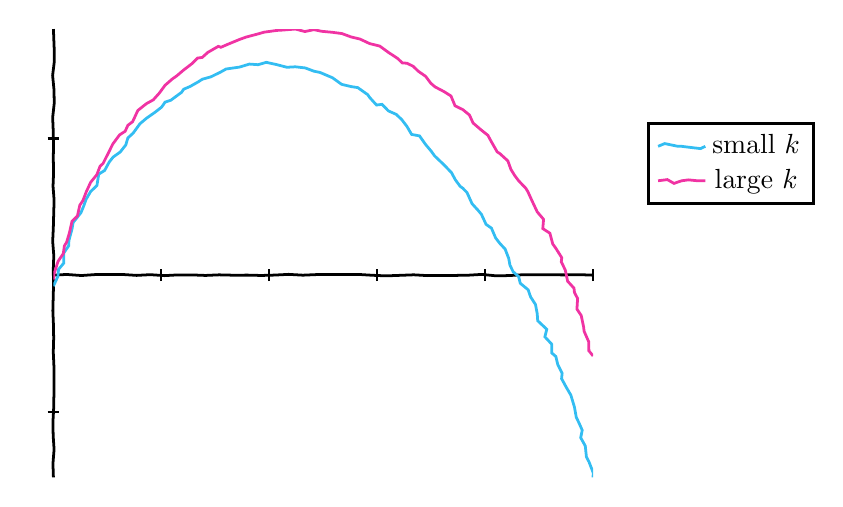
\begin{tikzpicture}[decoration={random steps,segment length=1mm,amplitude=0.2pt}]
        \pgfplotsset{every axis/.append style={line width=1pt}}

        \begin{axis}
        [
            axis x line=middle,
            axis y line=middle,
            xticklabels={},
            yticklabels={},
            every inner x axis line/.append style={-},
            every inner y axis line/.append style={-},
            decoration={random steps,segment length=5pt,amplitude=0.3pt},decorate,
            every tick/.style={thick,black,decorate},
            legend style={at={(1.1,0.7)}, anchor=west}
        ]
            \begin{scope}
            [
                decoration={random steps,segment length=3pt,amplitude=1pt},
                decorate
            ]
                \addplot [cyan!80!white, samples=30, domain=0:1] {-x*log2(x)-(1-x)*log2(1-x) - 0.02 - 0.5*(x+0.2)^2};
                \addplot [magenta!80!white, samples=30, domain=0:1] {-x*log2(x)-(1-x)*log2(1-x) - 0.008 - 0.2*(x+0.2)^2};
                \legend{small $k$, large $k$}
            \end{scope}
        \end{axis}
        \end{tikzpicture}
        \end{center}
\end{enumerate}
\end{solution}


\section*{Curie-Weiss is Back}
The Hamiltonian of the Curie-Weiss model reads
\begin{equation*}
    \mathcal{H}\rdbrs{ \clbrs{ s_i }_{i=1}^N } = -\frac{1}{2N} \rdbrs{ {\sum s_i} }^2 - h \sum_i s_i \, .    
\end{equation*}
As we have seen in our first set of lectures, the free energy 
$
f(\beta,h) = -\frac{1}{\beta} \limit{N \to \infty} \log \rdbrs{ Z_N(\beta,h) }
$ 
of the model can be written (asymptotically) as
$
f(\beta,h) = \min_{m \in [-1,1]} ~\mathcal{F}_m (\beta,h,m),
$
with the free energy at fixed magnetization ${\cal F}_m(\beta,h,m)$ being given by:
\begin{equation*}
    \mathcal{F}_m (\beta,h,m) = -\frac{1}{2} m^2 - h m + \frac{1}{\beta}
    \sqbrs{ \frac{1+m}{2} \log \rdbrs{ \frac{1+m}{2} } + \frac{1-m}{2} \log \rdbrs{ \frac{1-m}{2} } }
\end{equation*}
and the equilibrium value of the magnetization is given by the minimizer $ m^* $:
\begin{equation*}
    \agbrs{ \frac{\sum_i s_i}{N} } = m^*
\end{equation*}
\begin{enumerate}[(a)]
\item 
        Plot the function $ \mathcal{F}_m(\beta,h,m) $ as a function of $ m $ in the two following cases: 
        (a) at $ h = 0 $ for different values of $ \beta $ larger and lower than one and 
        (b) at a value of $ \beta $ larger than $ 1 $ for different values (positive and negative) of $ h $. 
        Describe what you see in both cases.
\item 
        Show \footnote{
        It may be useful to use one of the two following identities:
        \begin{IEEEeqnarray*}{rCl}
            \atanh(x) &=& \frac{1}{2} \log \rdbrs{ \frac{1+x}{1-x} } \text{ or } \\
            H(m) &=& \log \rdbrs{ 2 \cosh \rdbrs{ \atanh(x) } } - x \atanh(x)
            = -\sqbrs{ \frac{1+m}{2} \log \rdbrs{ \frac{1+m}{2} } + \frac{1-m}{2} \log \rdbrs{ \frac{1-m}{2} } }
        \end{IEEEeqnarray*}
        } that the minimizer $ m^* $ is also the solution of the so-called ``self-consistent equation''
        \begin{equation*}
            m = \tanh(\beta(m+h)) \, .
        \end{equation*}
        Compute the value of $ m^* $ in the three following cases: 
        (a) $ h = 10^{-6} $ and $ \beta^{-1} $ between $ 0 $ and $ 2 $, 
        (b) $ h = -10^{-6} $ and $ \beta^{-1} $ between $ 0 $ and $ 2 $, and 
        (c) $ \beta = 1.5 $ and $ h $ between $ -1 $ and $ 1 $.
\item 
        We now focus on the behavior at $ \beta = 1.5 $ with $ h $ between $ 0.1 $ and $ 0.2 $: 
        how many solution to the self-consistent equations are they? 
        Which one is the correct one according to the Laplace method (plot the function $ \mathcal{F}_m (\beta,h,m) $ to answer this question).
\end{enumerate}
\begin{solution} $\,$ 
\begin{enumerate}[(a)]
\item   
        The plot of function $ \mathcal{F}_m(\beta, h, m) $ under $ h = 0 $ and $ \beta = 0.9,1,1.2,1.5 $
        \begin{figure}[H]
            \centering
            \includegraphics[width=300pt]{hw1/hw1_2(a)_1.pdf}
        \end{figure}
        At high temperature ($ \beta < 1 $), the curve has only one minimum at zero.
        At low temperature ($ \beta > 1 $), the curve has two local minimums symmetric around zero.
        There is a phase transition at $ \beta = 1 $.

        The plot of function $ \mathcal{F}_m(\beta, h, m) $ under $ \beta = 1.2 $ and $ h = -0.1, -0.05, 0, 0.03, 0.07 $
        \begin{figure}[H]
            \centering
            \includegraphics[width=300pt]{hw1/hw1_2(a)_2.pdf}
        \end{figure}
        Since $ \beta > 1 $, the minimum will drift away from zero.
        The number of local minimums can be one or two depending on $ \abs{h} $.
        If $ h < 0 $, the global minimum will be closer to $ -1 $, if $ h > 0 $, the global minimum will be closer to $ 1 $.
        When $ h $ moves pass zero, the global minimum changes sharply to another value with opposite sign.
\item   Since $ m^* $ is the minimizer of $ \mathcal{F}_m(\beta, h, m) $ on interval $ [-1, 1] $, we can take partial derivative of $ \mathcal{F}_m(\beta, h, m) $ w.r.t. $ m $ and set it to zero
        \begin{IEEEeqnarray*}{rCl}
            0 &=& \eval{ \fracp{ \mathcal{F}_m(\beta, h, m) }{m} }_{m=m^*}
            % &=& m - h + \frac{1}{\beta} \sqbrs{ \frac{1}{2} \log \rdbrs{ \frac{1+m}{2} } + \frac{1}{2} - \frac{1}{2} \log \rdbrs{ \frac{1-m}{2} } - \frac{1}{2} } \\
            = \eval{ -m - h + \frac{1}{\beta} \frac{1}{2} \log \rdbrs{ \frac{1+m}{1-m} } }_{m=m^*}
            = -m^* - h + \frac{1}{\beta} \atanh(m^*) \, .
        \end{IEEEeqnarray*}
        By rearranging the equation yields
        \begin{equation*}
            m^* = \tanh(\beta(m^*+h)) \, ,
        \end{equation*}
        which is exactly the self-consistent equation.
        Note that $ m^* $ is actually a function of inverse temperature $ \beta $ and magnetic field $ h $.

        The plot of function $ m^*(\beta, h) $ under $ h = \pm {10}^{-6} $ and $ \beta^{-1} \in (0, 2] $
        \begin{figure}[H]
            \centering
            \includegraphics[width=270pt]{hw1/hw1_2(b)_1,2.pdf}
        \end{figure}
        The plot of function $ m^*(\beta, h) $ under $ \beta = 1.5 $ and $ h \in [-1,1] $
        \begin{figure}[H]
            \centering
            \includegraphics[width=270pt]{hw1/hw1_2(b)_3.pdf}
        \end{figure}
\item 
        The plot of function $ \mathcal{F}_m(\beta, h, m) $ under $ \beta = 1.5 $ and $ h = 0.1, 0.2 $
        \begin{figure}[H]
            \centering
            \includegraphics[width=300pt]{hw1/hw1_2(c).pdf}
        \end{figure}
        For $ h = 0.1 $, there are two solutions, the right one has lower function value thus it is the correct one.
        For $ h = 0.2 $, there is only one solution, so it is the correct one.
\end{enumerate}
\end{solution}


\section*{Monte-Carlo-Markov-Chain}
Consider again the Hamiltonian of the Curie-Weiss model. 
A very practical way to sample configurations of $ N $ spins from the Gibbs probability distribution
\begin{equation*}
    P \rdbrs{ \clbrs{ s_i }_{i=1}^N; \beta, h } = \frac{ \exp \rdbrs{ -\beta \mathcal{H} \rdbrs{ \clbrs{ s_i }_{i=1}^N; h } } }{ Z_N(\beta, h) }
\end{equation*}
is the Monte-Carlo-Markov-Chain (MCMC) method, and in particular the Metropolis-Hastings algorithm. 
It works as follows:
\begin{enumerate}
\item   Choose a starting configuration for the $ N $ spins values $ s_i = \pm 1 $ for $ i=1,\ldots,N $.
\item   Choose a spin $ i $ at random. Compute the current value of the energy $ E_{\mathrm{now}} $ and the value of the energy $ E_{\mathrm{flip}} $ if the spins $ i $ is flipped (that is if $ S^{\mathrm{new}}_i = -S^{\mathrm{old}}_i $).
\item   Sample a number $ r $ uniformly in $ [0,1] $ and, if $ r < \ee^{\beta (E_{\mathrm{now}} - E_{\mathrm{flip}})} $ perform the flip (i.e. $ S^{\mathrm{new}}_i = -S^{\mathrm{old}}_i $) otherwise leave it as it is.
\item   Goto step 2.
\end{enumerate}
If one is performing this program long enough, it is guarantied that the final configuration ($ \clbrs{ S } $) will have been chosen with the correct probability.
\begin{enumerate}[(a)]
\item 
        Write a code to perform the MCMC dynamics, and start by a configuration where all spins are equal to $ 1 $. 
        Take $ h = 0 $, $ \beta = 1.2 $ and try your dynamics for a long enough time (say, with $ t_{\mathrm{max}} = 100 N $ attempts to flips spins) and monitor the value of the magnetization per spin $ m = \sum_i s_i/N $ as a function of time. 
        Make a plot for $ N=10,50,100,200,1000 $ spins. 
        Compare with the exact solution at $ N = \infty $. 
        Remarks? Conclusions?
\item 
        Start by a configuration where all spins are equal to $ 1 $ and take $ h = -0.1 $, $ \beta = 1.2 $.
        Monitor again the value of the magnetization per spin $ m = \sum_i s_i/N $ as a function of time. 
        Make a plot for $ N = 10,50,100,200,1000 $ spins.
        Compare with the exact solution at $ N = \infty $. 
        Remarks? Conclusions?
\end{enumerate}
\begin{solution} $\,$ 
Before we write the code, let's first review the Curie-Weiss model.
Since we may try different $ \beta, h, N $, to avoid confusion it is better to write them explicitly.
For any $ k \in \clbrs{ 1, \ldots, N } $, we can split the Hamiltonian as
\begin{IEEEeqnarray*}{rCl}
    \mathcal{H} \rdbrs{ \clbrs{ s_i }_{i=1}^N; h }
    &=& -\frac{1}{N} \sum_{i < j} s_i s_j - h \sum_{i=1}^N s_i \\
    &=& \underbrace{ -\frac{1}{N} \sum_{\substack{i > j \\ i \ne k, j \ne k}} s_i s_j - h \sum_{i \ne k} s_i }_{\text{do not contain } s_k} - \underbrace{ \frac{1}{N} s_k \sum_{i \ne k} s_i - h s_k }_{\text{contains } s_k}
\end{IEEEeqnarray*}
Suppose we flip the $ k $-th spin, then since the only difference is $ S^{\mathrm{new}}_k = -S^{\mathrm{old}}_k $
\begin{IEEEeqnarray*}{rCl}
    E_{\mathrm{now}} - E_{\mathrm{flip}}
    &=& \mathcal{H} \rdbrs{ \clbrs{ s_i^{\mathrm{old}} }_{i=1}^N; h } - \mathcal{H} \rdbrs{ \clbrs{ s_i^{\mathrm{new}} }_{i=1}^N; h } \\
    &=& \sqbrs{ - \frac{1}{N} s_k^{\mathrm{old}} \sum_{i \ne k} s_i^{\mathrm{old}} - h s_k^{\mathrm{old}} } - \sqbrs{ - \frac{1}{N} s_k^{\mathrm{new}} \sum_{i \ne k} s_i^{\mathrm{new}} - h s_k^{\mathrm{new}} } \\
    &=& \sqbrs{ - \frac{1}{N} s_k^{\mathrm{old}} \sum_{i \ne k} s_i^{\mathrm{old}} - h s_k^{\mathrm{old}} } - \sqbrs{ \frac{1}{N} s_k^{\mathrm{old}} \sum_{i \ne k} s_i^{\mathrm{old}} + h s_k^{\mathrm{old}} } \\
    &=& -2 s_k^{\mathrm{old}} \sqbrs{ \frac{1}{N} \sum_{i \ne k} s_i^{\mathrm{old}} + h }
\end{IEEEeqnarray*}
Secondly, when $ N \to \infty $, the Boltzmann distribution is dominated by configurations whose magnetization equals $ m^* $.
So if we can run a simulation with infinite $ N $, the trace plot will start with a warm-up stage to reach $ m^* $, once $ m^* $ is reached, the trace plot will get stuck at there.
\begin{enumerate}[(a)]
\item 
        Since $ h = 0 $, there the two local minimizers have same function value so either one can achieve the global minimum.
        However, we start our MCMC chain at all-one configuration, which is closer to the positive minimizer.
        It is possible that the random walk will reach the negative minimizer.
        Actually in the long run, the chain will first walk to the positive minimizer and stay for a while, then walk to the negative minimizer and stay for a while, and do this back and forth.
        The larger $ N $ is, the longer the chain stay at the minimizers, and the less fluctuation the chain will deviated from the minimizer.
        \begin{figure}
            \centering
            \includegraphics[width=500pt]{hw1/hw1_3(a).pdf}
            \caption{Trace plot for $ \beta = 1.2, h = 0 $ and $ N = 10, 50, 100, 200, 1000 $}
        \end{figure}
\item 
        In this case we have similar behavior as part (a), the only difference is $ h = -0.1 $ breaks down the balance between two local minimizers.
        As discussed in Problem 2 (c), the negative minimizer is the correct one according to the Laplace method.
        So the trace plot will start with a warm-up stage to reach $ m^* $, once $ m^* $ is reached, the trace plot will get stuck at there.
        The larger $ N $ is, the less fluctuation the chain will deviated from $ m^* $.
        \begin{figure}
            \centering
            \includegraphics[width=500pt]{hw1/hw1_3(b).pdf}
            \caption{Trace plot for $ \beta = 1.2, h = -0.1 $ and $ N = 10, 50, 100, 200, 1000 $}
        \end{figure}
\end{enumerate}
\end{solution}

\end{document}